%% Преамбула TeX-файла

% 1. Стиль и язык
\documentclass[utf8x, 12pt]{G7-32} % Стиль (по умолчанию будет 14pt)


% Остальные стандартные настройки убраны в preamble.inc.tex.
\sloppy

% Настройки стиля ГОСТ 7-32
% Для начала определяем, хотим мы или нет, чтобы рисунки и таблицы нумеровались в пределах раздела, или нам нужна сквозная нумерация.
\EqInChapter % формулы будут нумероваться в пределах раздела
\TableInChapter % таблицы будут нумероваться в пределах раздела
\PicInChapter % рисунки будут нумероваться в пределах раздела

% Добавляем гипертекстовое оглавление в PDF
\usepackage[
bookmarks=true, colorlinks=true, unicode=true,
urlcolor=black,linkcolor=black, anchorcolor=black,
citecolor=black, menucolor=black, filecolor=black,
]{hyperref}

% Изменение начертания шрифта --- после чего выглядит таймсоподобно.
% apt-get install scalable-cyrfonts-tex

\IfFileExists{cyrtimes.sty}
    {
        \usepackage{cyrtimespatched}
    }
    {
        % А если Times нету, то будет CM...
    }

\usepackage{graphicx}   % Пакет для включения рисунков
\DeclareGraphicsExtensions{.jpg,.pdf,.png}
\graphicspath{{inc/img/}}
% С такими оно полями оно работает по-умолчанию:
\RequirePackage[left=20mm,right=10mm,top=20mm,bottom=20mm,headsep=0pt]{geometry}
% Если вас тошнит от поля в 10мм --- увеличивайте до 20-ти, ну и про переплёт не забывайте:
\geometry{right=20mm}
\geometry{left=30mm}



% Произвольная нумерация списков.
\usepackage{enumerate}

\setcounter{tocdepth}{1} %Подробность оглавления
%4 это chapter, section, subsection, subsubsection и paragraph
%3 это chapter, section, subsection и subsubsection
%2 это chapter, section, и subsection
%1 это chapter и section
%0 это chapter.


\begin{document}

%\frontmatter % выключает нумерацию ВСЕГО; здесь начинаются ненумерованные главы: реферат, введение, глоссарий, сокращения и прочее.
\begin{center} 

\large МГУ им. Ломоносова, факультет ВМК\\[5.5cm] 

\huge Курсовая работа \\[0.6cm] % название работы, затем отступ 0,6см
\large на тему:  <<Нейросетевые методы поиска и сегментации объектов в данных современных 
космических обзоров (eROSITA, ART-XC)>>\\[3.7cm]


\end{center} 

\begin{flushright}
Выполнила: студентка гр. 320 \\
Немешаева Алиса \\
\end{flushright}


\vfill 

\begin{center} 
\large Москва 2020
\end{center} 

\thispagestyle{empty}


\thispagestyle{empty}
\setcounter{page}{0}
\tableofcontents
\clearpage

\Annotation

Данная работа рассматривает возможность применения нейросетевых методов к решению проблемы 
сегментации и детекции объектов по многоволновым данным космических телескопов (в данном случае 
оптического, микроволнового и рентгеновского диапазонов). В качестве основы для нейросетевой 
архитектуры использовалась модель U-net. В итоге были реализованы алгоритмы по генерации 
искуственных данных, создан образец нейросети, обученной на таких данных и начата обработка 
настоящих данных оптического диапазона.\\

\Introduction
%Что дает сегментация разных диапазонов
%Отличие скоплений в оптике и рентгене
\section{Скопления галактик}
В 2019 году произошел запуск космической обсерватории СРГ (Спектр-Рентген-Гамма) с телескопами 
eROSITA и ART-XC на борту. Основной задачей этих телескопов является создание обзора всего неба в 
рентгеновском диапазоне. Данные, полученные от этих телескопов будут использоваться для обнаружения 
астрономических объектов трёх категорий:

\begin{enumerate}
    \item Скопления галактик.
    \item Сверхмассивные чёрные дыры.
    \item Рентгеновские звёзды в галактике Млечный путь. 
\end{enumerate}

Наибольший интерес представляют скопления галактик. Скопления --- это гравитационно связанные 
системы, которые являются самыми большими динамически связанными структурами во Вселенной. 
Скопления галактик играют важную роль в задачах определения космологических параметров Вселенной. 
Например, зная расстояние до скопления и его красное смещение (параметр, по которому можно понять, 
как объект отдаляется от наблюдателя), можно уточнить постоянную Хаббла, входящую в закон Хаббла, 
который описывает скорость расширения Вселенной. Кроме того, соотношение компонент материи в 
скоплениях должно отражать средний состав Вселенной, что позволяет измерить вклад барионов в общую
плотность Вселенной.\\
Скопления галактик излучают энергию в разных диапазонах, и 
их можно наблюдать не только в рентгеновских данных.\\

\begin{figure}[h]
    \center{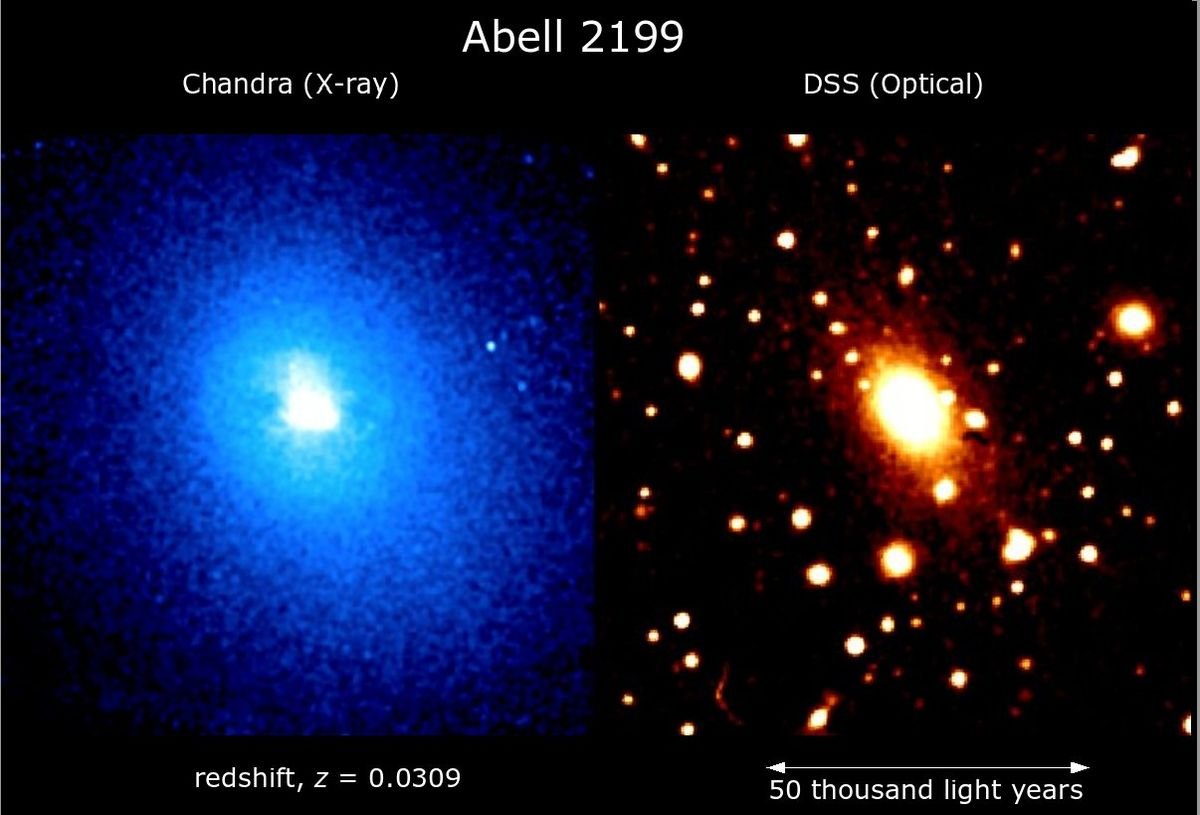
\includegraphics[width=0.7\linewidth]{comparison0}}
    \caption{Скопление <<Абель 2199>> в оптическом и рентгеновском диапазонах. \cite{Abell}}
\end{figure}

Полные обзоры неба, полученные телескопом eROSITA, появятся к июню 2020 года, поэтому на данный 
момент есть возможность подготовить модели для сегментации данных на примере других диапазонов.\\

В первую очередь будут использоваться данные оптического диапазона. Видимое излучение --- тот 
диапазон частот, что доступен глазу человека. На текущий момент существует большое количество 
оптических телескопов, и, как следствие, большое количество данных, извлеченных с их помощью. В 
данной работе будут использоваться данные телескопа Pan-STARRS1, который является частью системы 
телескопов Pan-STARRS (Panoramic Survey Telescope and Rapid Response System). Этот телескоп 
построен на вершине гавайского вулкана Халеакала. На 2007 год он обладал самой большой 
светочувствительной матрицей в мире. Кроме того, его данные находятся в общем доступе \cite{Panstarrs}.\\

\section{Нейросетевые методы}
В последние годы методы глубокого обучения стали играть важную роль в анализе данных. Нейросетевые 
модели показывают высокие результаты в области компьютерного зрения и в частности в задачах 
сегментации и детекции. Всё более часто они применяются и для решения задач астрофизики. 
Характеристики телескопа eROSITA позволят получить рентгеновские данные очень высокого качества (то 
есть с низким количеством шума), и методы глубокого обучения дают много преимуществ при анализе 
данных: 

\begin{enumerate}
    \item Стандартные алгоритмы сегментации усредняют информацию по нескольким каналам,
        в то время как с помощью нейросети можно охватить данные полностью и исследовать вопрос с 
        новой стороны. Таким образом, нейросеть будет получать <<сырые>> данные, что экономит время 
        и исключает необходимость контролировать процесс предобработки данных. 
        Кроме того, нейросеть, используя все данные, может получить информацию о 
        калибровке телескопа прямо из обзоров, что невозможно сделать при использовании классических 
        методов.
    \item Аналогичнные методы можно использовать для сегментации одновременно разнородных данных. 
        То есть для улучшения качества сегментации можно исследовать параллельно разные диапазоны 
        частот и находить взаимосвязь между разными спектрами.
    \item Каждый из классических методов имеет свои достоинства и недостатки, и для каждого 
        диапазона излучения существуют свои алгоритмы, в то время как 
        нейросеть может стать универсальным средством для сегментации.
\end{enumerate}

U-net \cite{Unet} является стандартной архитектурой для сегментации данных. Она идеально подходит 
для проверки идеи использования методов глубокого обучения для сегментации скоплений.
Её симметричная структура позволяет абстрагировать данные изображения, подаваемого на 
вход, в то время как skip-connection слои помогают увеличивать точность сегментации.

\begin{figure}[h]
    \center{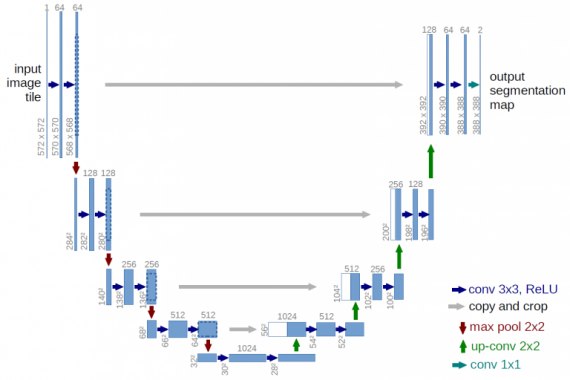
\includegraphics[width=0.7\linewidth]{unet0}}
    \caption{Структура модели U-net \cite{Unet}}
\end{figure}




\mainmatter

\chapter{Постановка задачи}
\label{cha:ch_1}

Задача состоит в исследовании и разработке нейросетевой модели, позволяющей выполнять сегментацию 
и впоследствии детекцию скоплений галактик на оптических данных.\\


\chapter{Обзор существующих решений рассматриваемой задачи или её модификаций}
\label{cha:ch_2}

\chapter{Исследование и построение решения задачи}
\label{cha:ch_3}

\section{План работы}
Для достижения цели задание было разделено на несколько шагов:

\begin{enumerate}

    \item Изучение архитектуры сегментации.
    \begin{enumerate}
        \item Выбор архитектуры для сегментации.
        \item Создание образца модели U-net.
    \end{enumerate}

    \item Обработка данных PS1.
    \begin{enumerate}
        \item Симуляции.
        \begin{enumerate}
            \item Создание простейших симуляций данных со скоплениями.
        \end{enumerate}
        \item Данные PS1.
        \begin{enumerate}
            \item Загрузка и обработка данных о скоплениях.
            \item Генерация <<патчей>> --- небольших областей неба, на которых будет тренироваться нейросеть.
            \item Загрузка и обработка обзоров неба PanSTARRS1 из области патчей.
            \item Преобразование данных PanSTARRS1 в двумерные матрицы для загрузки в нейросеть.
        \end{enumerate}
    \end{enumerate}

    \item Создание модели и подбор параметров.
    \begin{enumerate}
        \item Проверка работы U-net на данных симуляций.
        \item Обучение модели, подбор параметров модели (количество слоёв, методы аугментации, размер 
            батча, количество эпох обучения)
        \item Тестирование модели на заранее выбранных данных.
    \end{enumerate}

    \item Постобработка данных и проверка результатов.
    \begin{enumerate}
        \item Преобразование масок сегментации в координаты (детектирование скоплений).
        \item Сравнение полученных скоплений с существующими каталогами.
    \end{enumerate}
\end{enumerate}

\section{Особенности данных}
Матрицы, получающиеся при преобразовании данных из космических 
координат, обычно получаются разреженными и для них приходится использовать значения с плавающей 
точкой. Более того, нужно учитывать точность преобразования и выбирать достаточно детализированное 
разбиение проекции на пиксели изображения, иначе разные объекты могут слиться в один. Угловой 
размер области тоже имеет значение, так как на слишком маленьких частях неба искать такие большие 
объекты, как скопления галактик, бессмысленно.\\


\section{Создание симуляций}
Для создания симуляций использовался простейший алгоритм с использованием генерации случайных 
данных. По предположению данные скоплений можно аппроксимировать равномерным, пуассоновским и 
гауссовым распределениями.
Поэтапно создание симулированных данных выглядит так:

\begin{enumerate}
	\item Равномерным распределением создаём заданное количество скоплений на изображении.
	\item Для каждого скопления выбираем размер и количество объектов из распределения Пуассона.
	\item Для каждого скопления координаты объектов генерируются из распределения Гаусса.
	\item Равномерно генерируются координаты объектов шума.
\end{enumerate}

\begin{figure}[h]
    \center{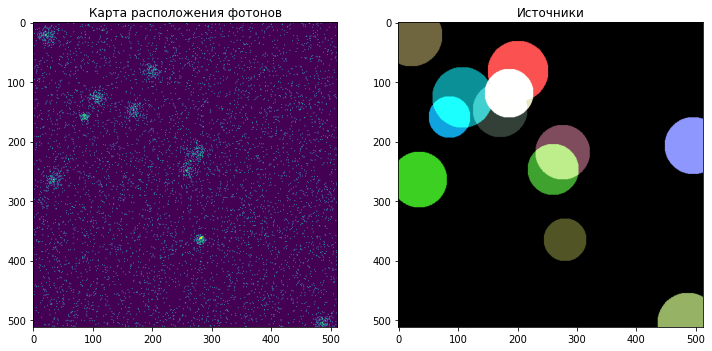
\includegraphics[width=0.7\linewidth]{gen0}}
    \caption{Пример генерации симулированных данных со скоплениями}
\end{figure}


\section{Обработка данных PS1}
Так же, как и в статье \cite{Bonjean}, в качестве списка скоплений будем использовать каталог PSZ2. 
Аналогичным образом будем генерировать патчи для создания тренировочных, валидационных и тестовых 
выборок (в том числе для валидации и тестирования будут выбраны те же пиксели разбиения $n_{side}=2$. 
Патчи выбирались так, чтобы в их окрестности находилось хотя бы одно из скоплений нужного каталога. 
После этого в базе данных PS1 (Pan-STARRS1) запрашивался список объектов, подходящих под заданные 
условия. \\

Для каждого объекта из PS1 загружались следующие данные:
\begin{enumerate}
    \item id объекта.
    \item Координаты объекта.
    \item (filter)PSFFlux - информация о ядре объекта.
    \item (filter)PSFFluxErr - ошибка измерения (filter)PSFFlux.
    \item (filter)KronFlux - информация о полном свете объекта.
    \item (filter)KronFluxErr - ошибка измерения (filter)KronFlux.
\end{enumerate}

Вместо (filter) подставляется одна из букв \{g, r, i, z, y\}, обозначающих фильтр, которым 
обрабатывалась информация об объектах. Таким образом, информация об излучении объекта хранится в 
20 параметрах, включая ошибки.\\

Из-за особенностей данных, некоторые объекты могут повторяться (то есть их координаты полностью 
совпадают). В таких ситуациях нужно провести слияение объектов --- для каждого из параметров 
(filter)PSFFlux и (filter)KronFlux нужно сохранить значение из той строки, где ошибка 
соответствующего измерения будет ниже. Оставшиеся значения ошибок можно либо удалить из данных, 
либо использовать их для аугментации: 
каждый раз при переносе значения какого-либо параметра, прибавлять к нему случайное значение из 
нормального распределения $N(0, (filter)(parameter)Err)$.\\

После того, как будут получены данные для обучения, их нужно из таблиц преобразовать в двухмерные 
матрицы изображений, чтобы создать выборки с количеством каналов, совпадающих с количеством 
исследуемых параметров у объектов. \\

Для примера, таблица с данными для 50 патчей содержит около 10 миллионов объектов. Обработка 
сотни объектов будет длится несколько минут, поэтому необходимо отдельно распараллелить процесс.\\

Для обучения планируется использование параметров (filter)KronFlux, то есть у первой версии 
нейросетевой модели будет 5 входных слоёв. Значения (filter)PSFFlux нужны для того, чтобы заменить 
ими отсутствующие измерения (filter)KronFlux для некоторых объектов.\\


\chapter{Проблема проекции неба на плоскость}
\label{cha:ch_4}

Существует несколько способов преобразовать данные, записанные как координаты объектов в космических
координатах, в значения на плоскости, которые можно уложить на двумерную матрицу. При любой проекции 
сферы на плоскость мы будем сталкиваться с искажениями в разной степени и для разных параметров данных.

\section{HEALPix}
Этот формат является очень удобной формой хранения данных. Данные телескопа <<Планк>>, исследование
которых упоминается в обзоре существующих решений, хранятся именно в этом формате, поэтому над ними 
легко работать и для них не требуется такое количество стадий предобработки, как например для данных 
PS1. \\

Как ранее было упомянуто, HEALPix является иерархической структурой для хранения данных. Она 
позволяет сохранить на проекции площадь объекта, однако его форма может быть искажена. Таким образом,
задавая маски скоплений как круги, мы в большинстве случаев будем наблюдать их искажение до эллипсов.\\

\begin{figure}
    \center{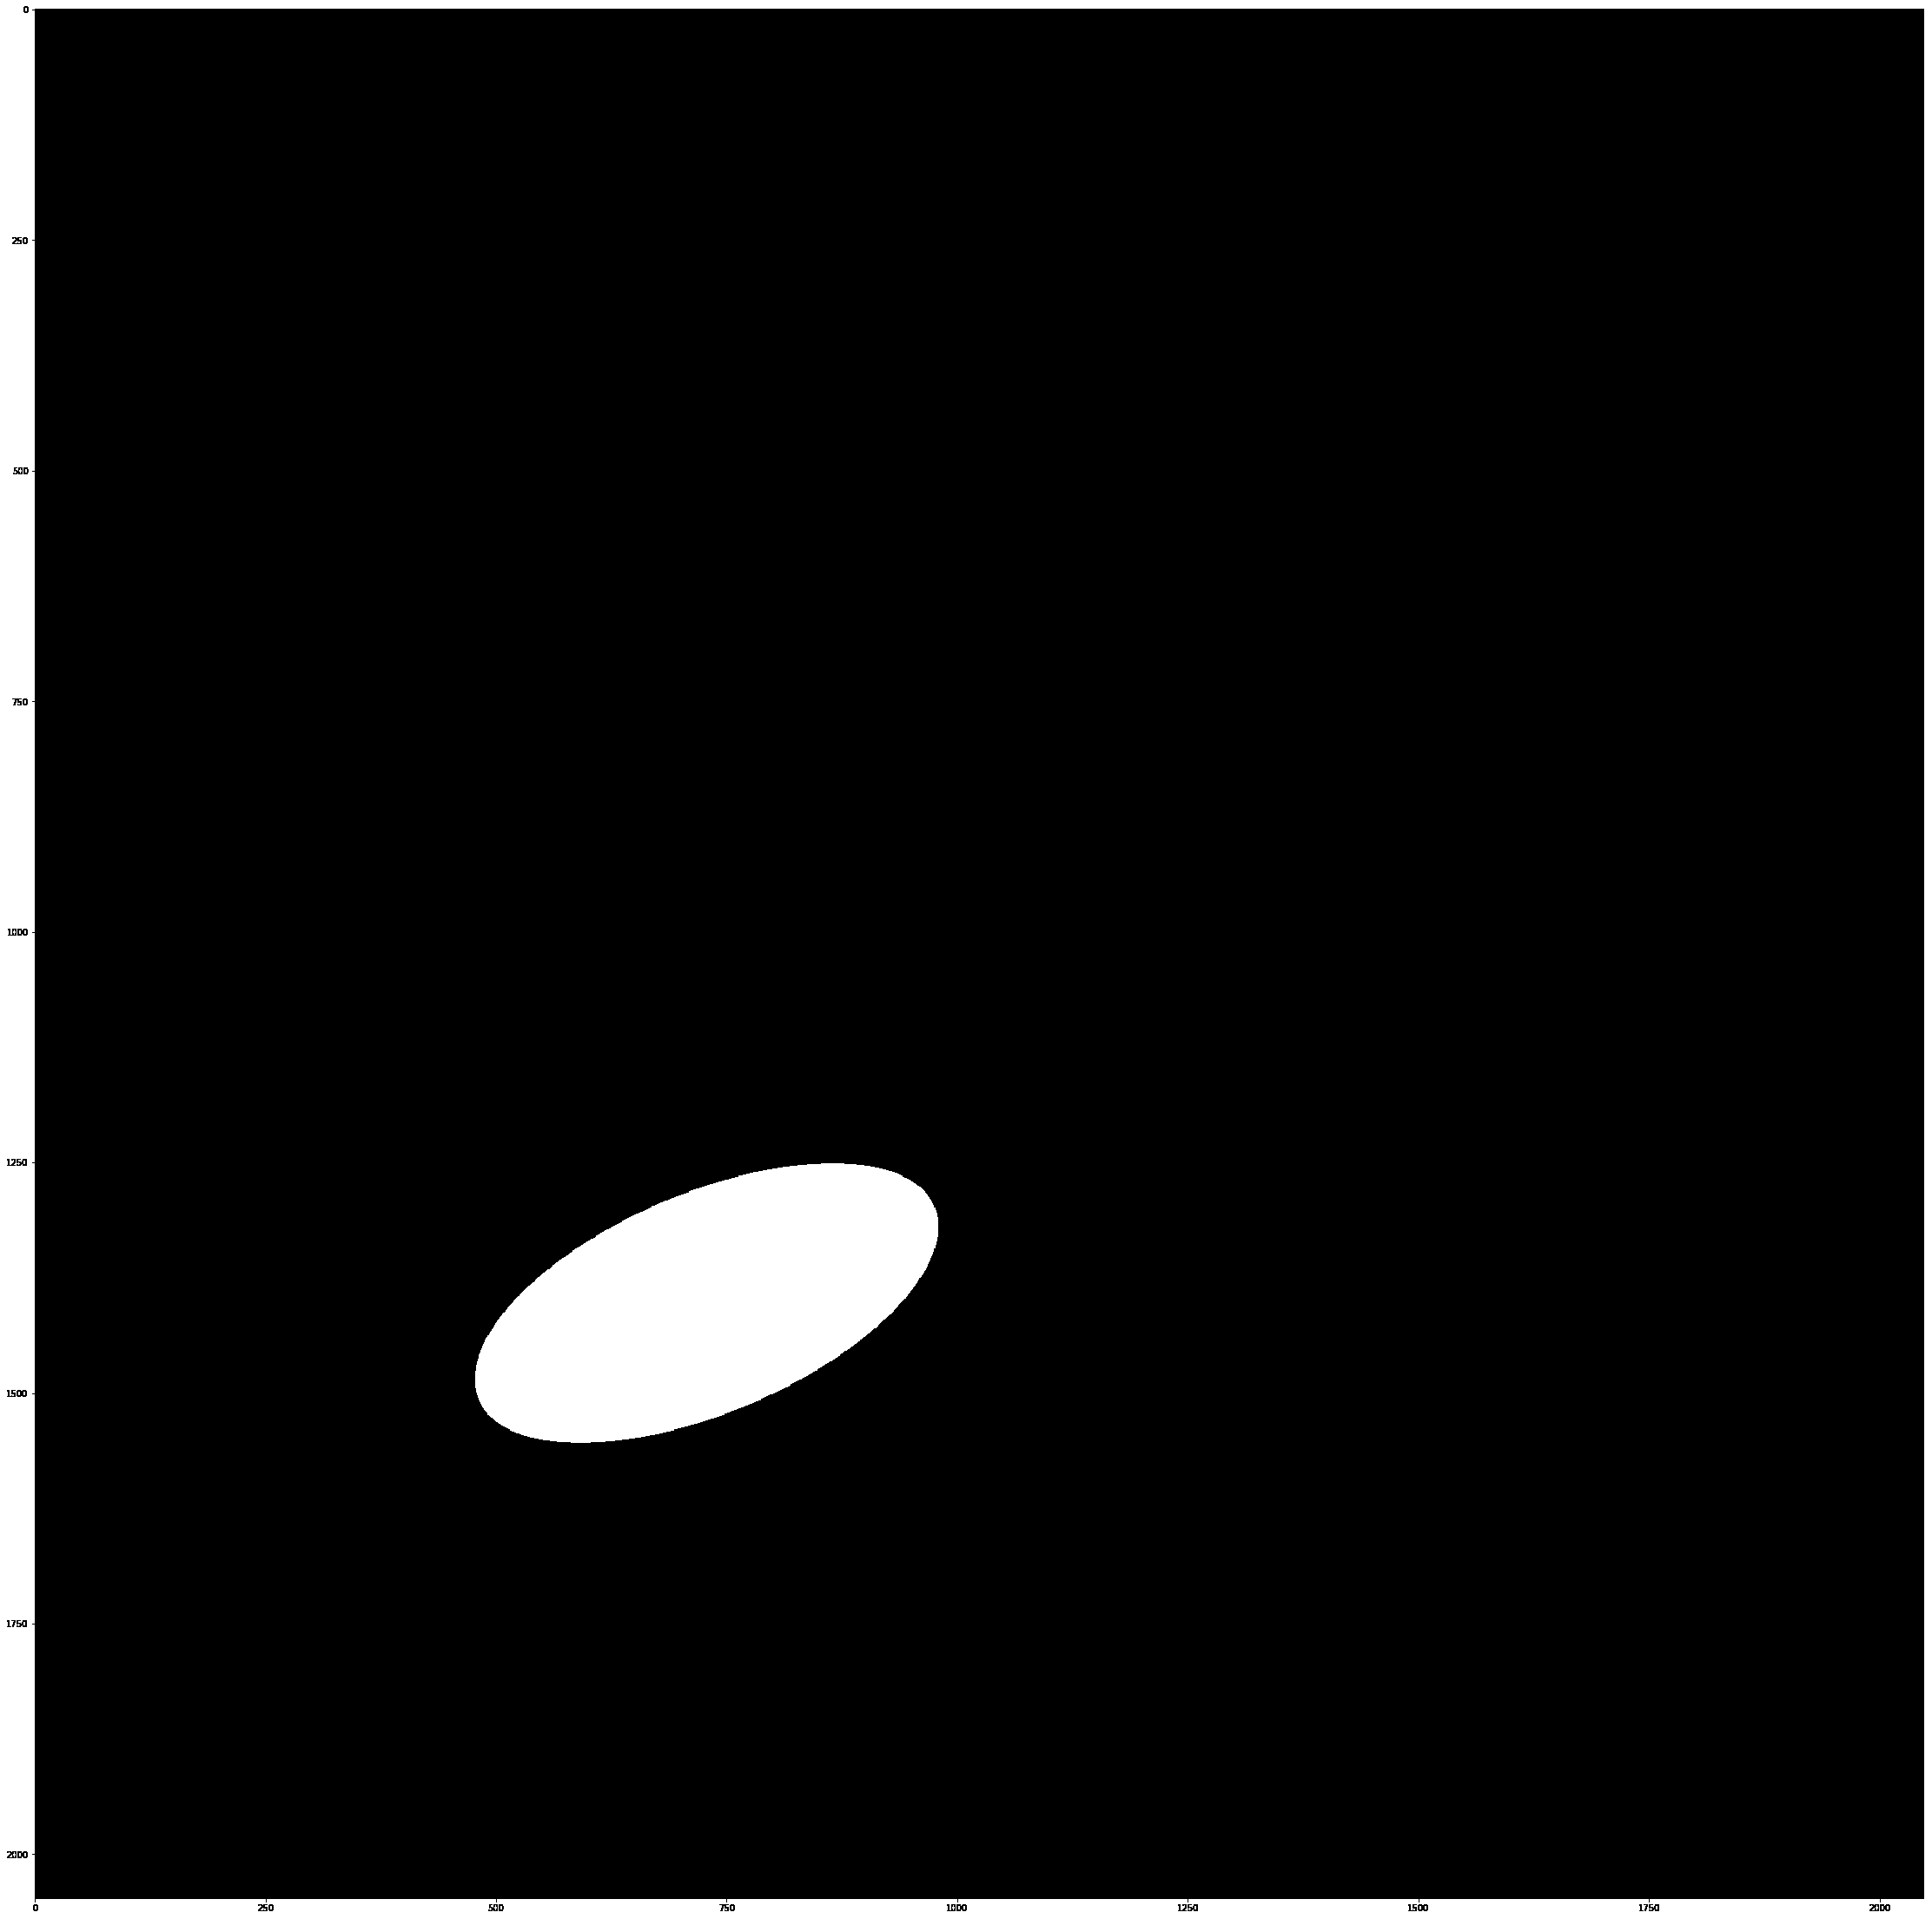
\includegraphics[width=0.6\linewidth]{mask0}}
    \caption{Пример маски для сегментации скопления. В разбиении с $n_{side} = 2^{17}$ были выбраны
        те пиксели, расстояние которых от центра скопления меньше $5'$}
\end{figure}

\section{Тангенциальная проекция}
Ещё один способ перенести данные со сферы на плоскость --- тангенциальная проекция WCS (World 
Coordinate Systems). Такая проекция сохраняет форму объектов, но искажает их площадь. Кроме того, 
такая проекция меняется в зависимости от выбранного центра проектирования объектов, и один и тот же
объект может попасть на разные проекции, что не всегда можно отследить. \\

Проекция HEALPix считается более удобной, так как она является абсолютной для всей области неба и 
для неё нет необходимости выбирать центр проекции.\\


\backmatter %% Здесь заканчивается нумерованная часть документа и начинаются ссылки и
            %% заключение

\Conclusion % заключение к отчёту

Текст заключения


\nocite{*}
\bibliographystyle{gost780u}
\bibliography{0-main}


\appendix   % Тут идут приложения

%\chapter{Первое Приложение}

\end{document}
